\section{Implementation}
\subsection{LSM tree}
An LSM tree, or log-structured merge-tree, is a key-value data structure with good performance characteristics. It is a good choice for providing indexed access to the data files, such as transaction log data or time series data. LSM tree maintains the data in two or more structures. Each of them is optimized for the media it is stored on, and the synchronization between the layers is done in batches~\cite{lsm_tree_orig}.

A simple LSM tree consists of two layers, named $C_0$ and $C_1$. The main difference between these layers is that typically $C_0$ is an in-memory data structure, while $C_1$ should be stored on a disk. Therefore, $C_1$ usually is bigger than $C_0$, and when the amount of data in $C_0$ reaches a certain threshold, the data is merged to $C_1$. To maintain a suitable performance it is suggested both $C_0$ and $C_1$ have to be optimized for their application. The data has to be migrated efficiently, probably using algorithms that may be similar to merge sort.

To maintain this merging efficiency, it was decided to use SSTable as the $C_1$ level, and B-tree for the $C_0$. SSTable, or Sorted String Table, is a file that contains key-value pairs, sorted by key~\cite{sstable}. Using SSTable for storing time series data is a good solution if the data is being streamed from a monitoring system. Because of this, they are sorted by the timestamp, which is a good candidate for the key. The value for the SSTable could be the measurement itself. SSTable is always an immutable data structure, meaning that the data cannot be directly deleted from the file; it has to be marked as "deleted" and then removed during the compaction process. The compaction process is also used to remove the obsolete data if it has a specific time-to-live period.

\subsection{Commitlog}
Any application that is used to work with mission-critical data has to have the ability to consistently save the data in case of a power outage or any other unexpected termination of the application. To maintain this ability, a commit log mechanism is used. It is a write-only log of any inserts to the database. It is written before the data is appended to the data files of the database. This mechanism is commonly used in any relational or non-relation DBMS.

Since the in-app storage system has to maintain this ability as well, it was necessary to implement the commit log alongside the LSM tree. In order to ensure that the entries in this commit log are persisted on the disk storage, the fsync syscall was used, which negatively affected the performance of the resulted storage system.

\subsection{Implemented library}
In order to implement the feature of storing time-series data within the Go application, the GoLSM library was developed. It provides mechanisms to persist and retrieve time-series data, and it uses a two-layer LSM tree as well as a commit log mechanism to store the data on disk. The architecture of this library is represented in Figure~\ref{fig2}.
\begin{figure}[h!]
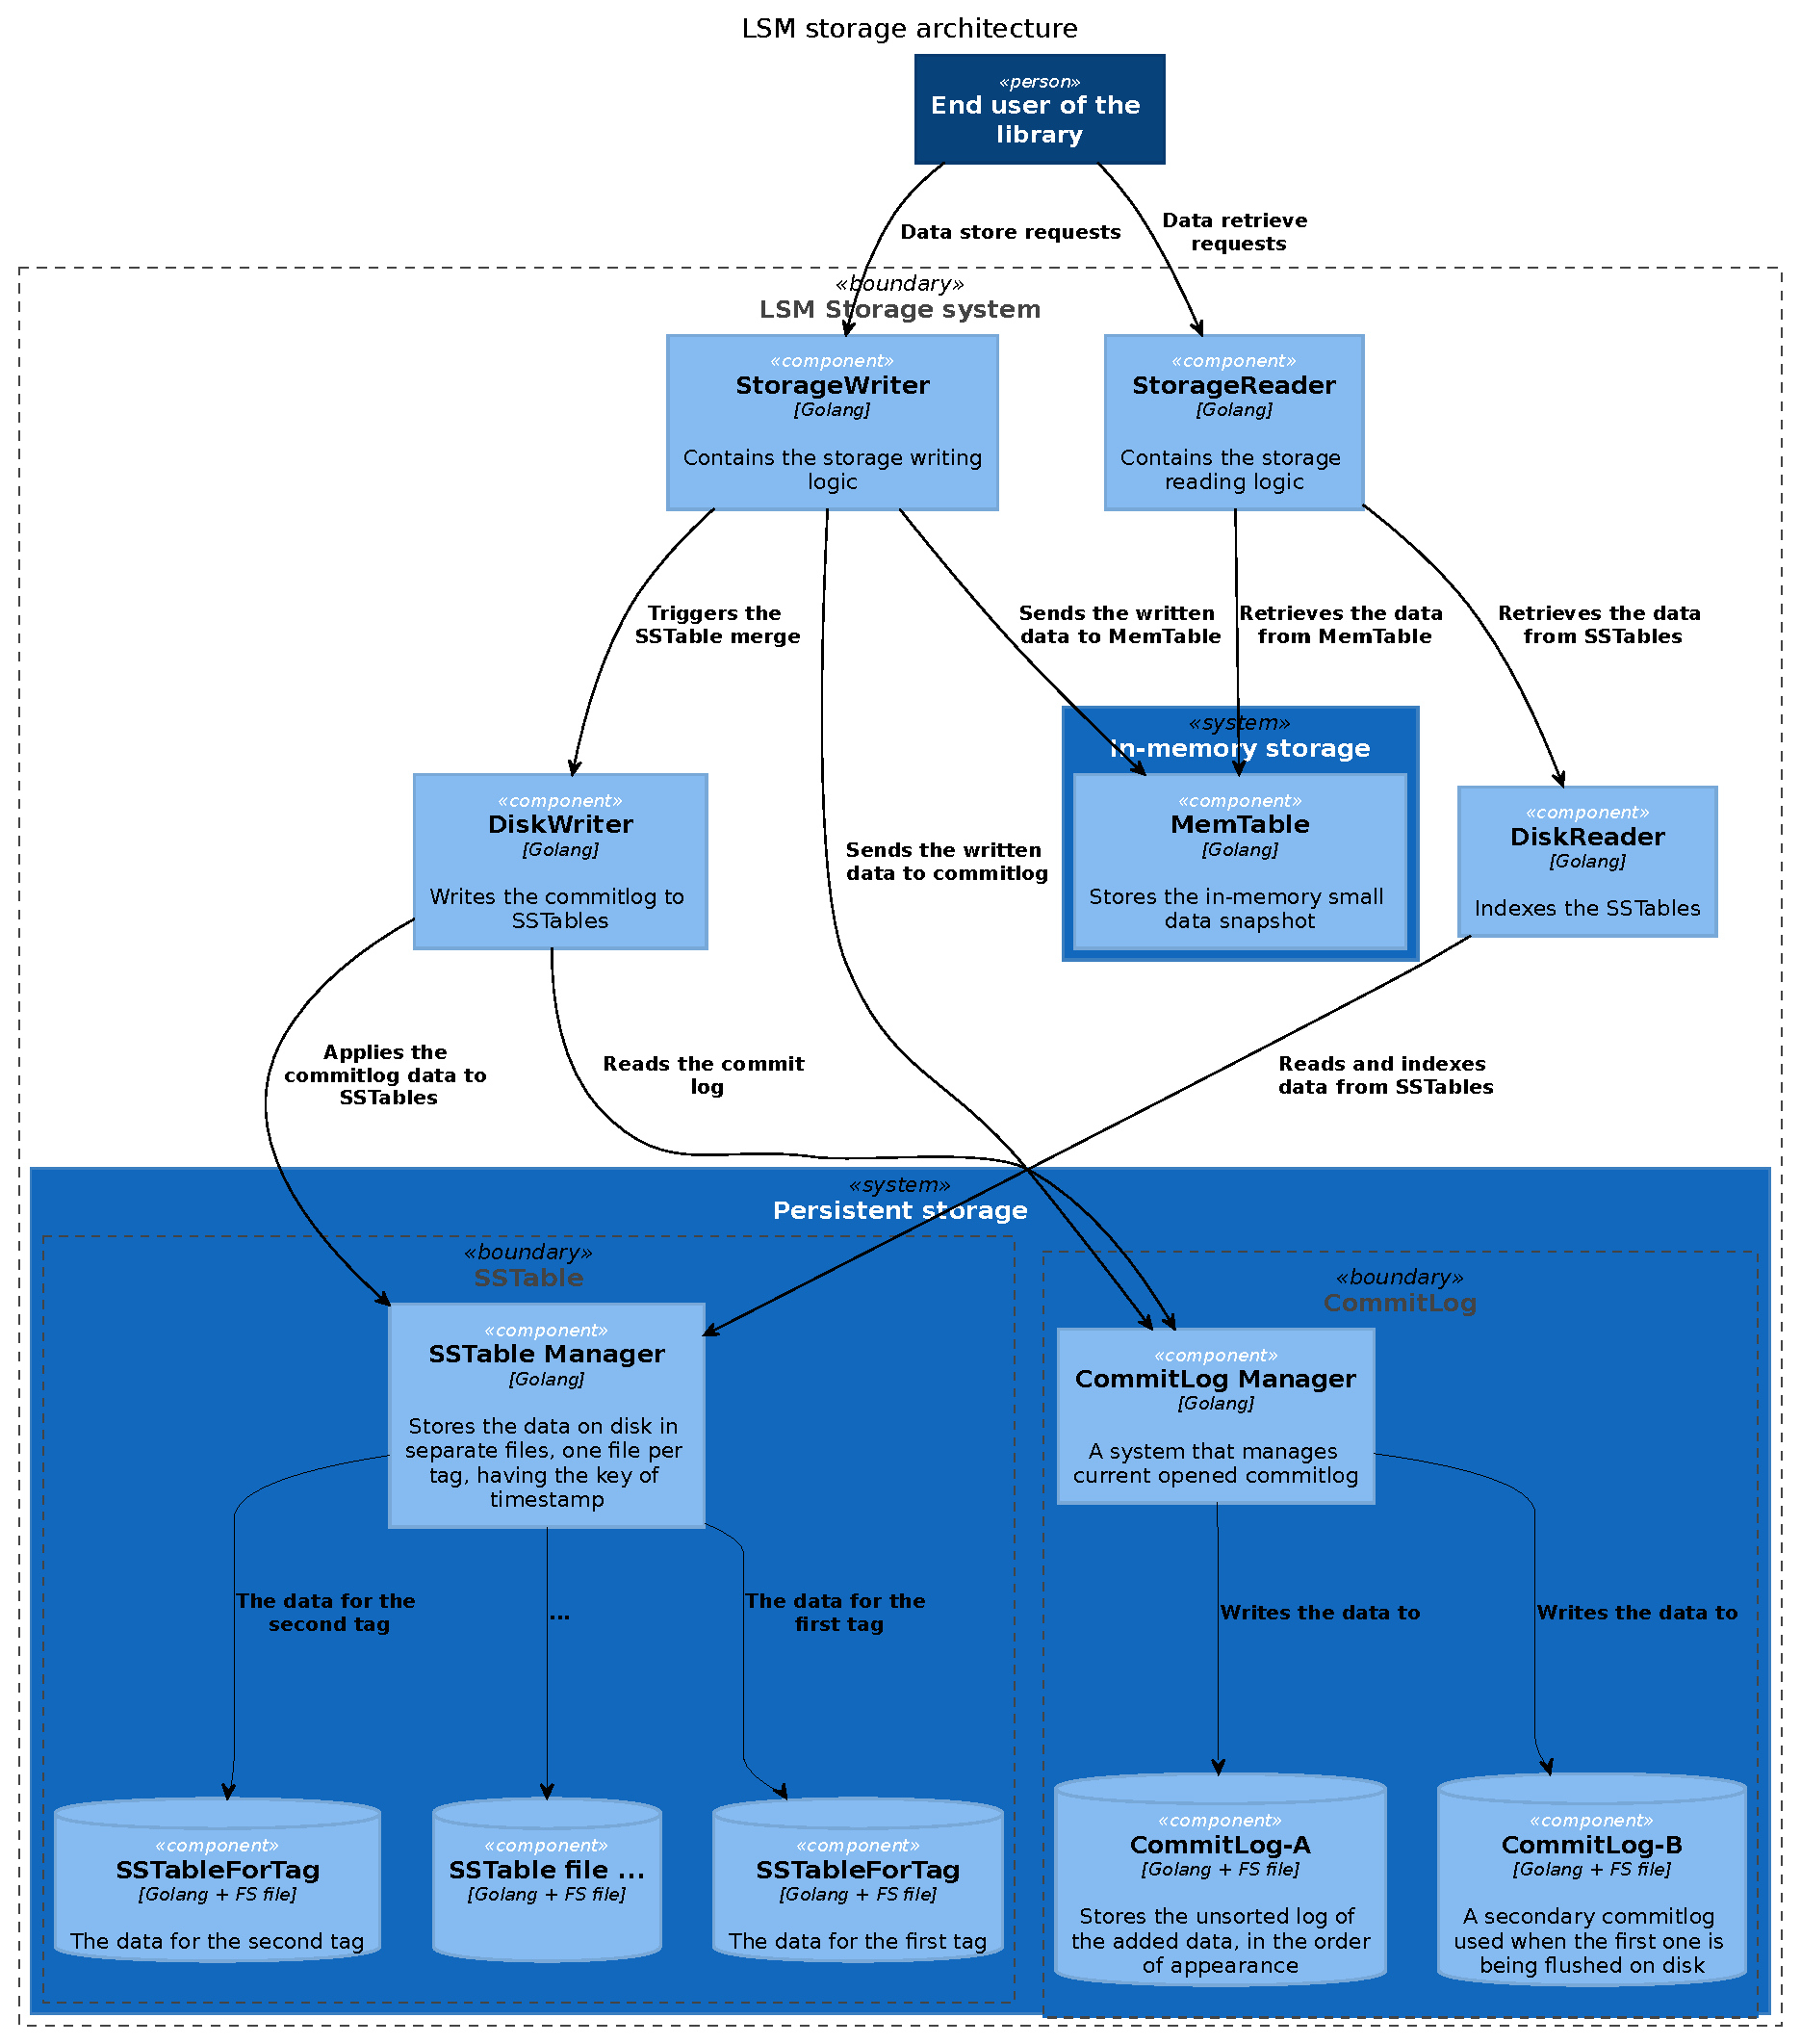
\includegraphics[width=\textwidth,keepaspectratio]{figures/golsm-arch.eps}
\caption{An architecture of a GoLSM library.} \label{fig2}
\end{figure}

 Since this library was initially developed for a particular subject area and particular usage, it has a number of limitations. For example, it has no functions to delete the data; instead, it is supposed to save the measurement with a particular expiration point, after which the data will be automatically removed during the compaction process. The data that is being stored using GoLSM should consist of one or multiple measurements; each measurement is represented by a tag name, which could be an identifier of a sensor or the measurement device, origin, which is the timestamp when the measurement was captured, and the measurement value, which is stored as a byte array. This byte array can vary in size. It makes the storage of each measurement a more complicated procedure.

As seen, the storage system consists of two layers, in-memory layer and persistent storage layer. The in-memory layer is based on a B-tree implementation by Google~\cite{btree_google} . It stores a small portion of the data of a configurable size. The storage layer consists of a commit log manager and an SSTable manager. The commit log manager maintains the two commit log files; while one is used to write the current data, another one is used to append the previously written data to the SSTable files, which are managed by SSTable Manager. Each SSTable file contains its own tag, and it also has a dedicated in-memory index, which is also based on a B-tree. This index is used to speed up the retrieval of the data from the SSTable when the requested time range is bigger than what is stored on an in-memory layer.